\documentclass[14pt]{extarticle}
\usepackage{fontspec}
\usepackage{geometry}
\geometry{a4paper, margin=2.1cm}
\usepackage{graphicx}
\usepackage{booktabs}
\usepackage{array}
\usepackage{amsmath}
\usepackage{amssymb}
\usepackage[table]{xcolor}
\usepackage{titlesec}
\usepackage{fancyhdr}
\usepackage{enumitem}
\usepackage[most]{tcolorbox}

\definecolor{theme}{HTML}{2b6a77}
\definecolor{ink}{HTML}{232d33}
\definecolor{ok}{HTML}{3f8161}
\definecolor{warn}{HTML}{b5651d}
\definecolor{cardbg}{HTML}{f3f6f7}
\definecolor{softgray}{HTML}{eef1f2}

\setmainfont{THSarabunNew.ttf}[
  Path=./fonts/, BoldFont=THSarabunNew Bold.ttf,
  ItalicFont=THSarabunNew Italic.ttf, BoldItalicFont=THSarabunNew BoldItalic.ttf]
\setmonofont{cour.ttf}[Path=./fonts/, BoldFont=courbd.ttf, Scale=0.82]
\XeTeXlinebreaklocale "th"
\XeTeXlinebreakskip = 0pt plus 0.1pt

\titleformat{\section}{\Large\bfseries\color{theme}}{\thesection.}{0.5em}{}
\titleformat{\subsection}{\large\bfseries\color{ink}}{\thesubsection}{0.5em}{}
\setlist{itemsep=1pt, topsep=2pt}
\pagestyle{fancy}\fancyhf{}
\fancyhead[L]{\small\color{ink} CL-7 · Spatial Profile \& Plateau Resolution}
\fancyhead[R]{\small\color{ink}\thepage}
\renewcommand{\headrulewidth}{0.4pt}
\newcommand{\code}[1]{{\ttfamily\detokenize{#1}}}
\newtcolorbox{keybox}{colback=cardbg, colframe=theme!55, boxrule=0.8pt, arc=2pt, left=8pt, right=8pt, top=5pt, bottom=6pt}

\begin{document}

\begin{center}
{\LARGE\bfseries\color{theme} รายงานการทดสอบสมมติฐาน CL-7}\\[3pt]
{\Large Spatial Profile \& Plateau Resolution}\\[5pt]
{\small การตรวจจับรอยแตกด้วยลายเซ็นการกระเจิง (SPR) --- OpenGATE 10 / Geant4}\\
{\small รายงานเฉพาะการทดสอบ CL-7 (วิเคราะห์ข้อมูลเดิม) \quad$\bullet$\quad \today}
\end{center}
\vspace{2pt}{\color{theme!45}\hrule}\vspace{8pt}

\section*{บทคัดย่อ}
CL-7 ตอบปมที่ CL-1 ทิ้งไว้: ``ภาวะอิ่มตัว (plateau) ระหว่าง 0.54 กับ 1.0~มม.\ เกิดจาก ROI ขนาดคงที่
เจือจางสัญญาณ หรือเป็นการอิ่มตัวเชิงกายภาพ'' โดยวิเคราะห์\textbf{โปรไฟล์เชิงพื้นที่}และ\textbf{สัญญาณรวม
(integrated)} บนข้อมูล CL-0 (ไม่รันใหม่) ผลสรุป: \textbf{สัญญาณรวมก็อิ่มตัวเช่นกัน} (0.54 เทียบ 1.0
ต่างกันไม่มีนัยสำคัญ, $p=0.73$) $\Rightarrow$ \textbf{plateau เป็นของจริงเชิงกายภาพ มิใช่สิ่งประดิษฐ์ของ ROI}
--- SPR ตรวจ\textbf{การมีอยู่}ของรอยแตกได้ไวมาก (ถึง 0.3~มม.) และมี dose--response ในช่วง $<0.5$~มม.
แต่\textbf{ความไวต่อความกว้าง}ของรอยแตกอิ่มตัวเกิน $\sim$0.5~มม.

\section{สมมติฐานและขอบเขต}
\textbf{ปมจาก CL-1:} plateau (0.54 vs 1.0) แยกไม่ออกด้วย ROI-mean และการเพิ่ม seed ไม่คุ้ม ($\sim$111 seeds)
CL-1 เสนอว่าอาจเป็นเพราะ ROI ขนาดคงที่ ``เจือจาง'' สัญญาณของร่องที่กว้างขึ้น\\
\textbf{สมมติฐาน CL-7:} ถ้า plateau เป็นเพราะ ROI เจือจาง $\Rightarrow$ \textbf{สัญญาณรวม (integrated)}
ซึ่งไม่ขึ้นกับการเฉลี่ย ควรยังโตตามขนาด; ถ้าสัญญาณรวมก็อิ่มตัว $\Rightarrow$ เป็นการอิ่มตัวเชิงกายภาพ\\
\textbf{ข้อมูล:} แผนที่ $\Delta$SPR ต่อ seed ของ 4 ขนาดจาก CL-0 (8 seeds) --- วิเคราะห์ล้วน ไม่รันใหม่

\section{วิธีวิเคราะห์}
\begin{enumerate}
  \item \textbf{Radial profile:} เฉลี่ย $\Delta$SPR ในวงแหวนรัศมี $r$ รอบจุดร่อง (เฉพาะในลำแสงสะอาด $r<9$)
        เพื่อดูรูปทรงและความลึกของแอ่ง
  \item \textbf{Integrated signal:} $-\sum\Delta\mathrm{SPR}$ ในดิสก์ $r<8$ ต่อ seed $\to$ mean\,$\pm$\,SEM
        (8 seeds) --- ตัวชี้วัดสัญญาณรวมที่ไม่ถูกเจือจางแบบค่าเฉลี่ย
  \item \textbf{Plateau test:} เทียบ integrated ของ 1.0 vs 0.54 แบบจับคู่ต่อ seed
\end{enumerate}

\section{ผลการวิเคราะห์}

\begin{table}[h]\centering\small
\renewcommand{\arraystretch}{1.3}
\begin{tabular}{c c c}
\rowcolor{softgray}
ขนาด & integrated $-\Delta$SPR ($\times10^{-3}$) & ROI-mean $|t|$ (CL-0) \\
\midrule
0.306 มม. & $5.3\pm2.1$ & 3.12 \\
0.43 มม.\  & $8.2\pm1.9$ & 3.66 \\
0.54 มม.\  & $\mathbf{10.4\pm2.4}$ & 4.84 \\
1.0 มม.\   & $9.4\pm1.6$ & 4.32 \\
\bottomrule
\end{tabular}
\end{table}
\vspace{-3pt}
\textbf{ทั้งสองตัวชี้วัดให้รูปแบบเดียวกัน} --- โตในช่วง 0.306$\to$0.54~มม.\ แล้วอิ่มตัว

\subsection{โปรไฟล์เชิงรัศมีของแอ่ง}
ทุกขนาดมีแอ่ง $\Delta$SPR ที่จุดร่อง ฟื้นสู่ 0 ภายใน $\sim$6px รูปทรงคล้ายกัน โดยลึกสุดที่ $\sim$0.5~มม.

\begin{figure}[h]\centering
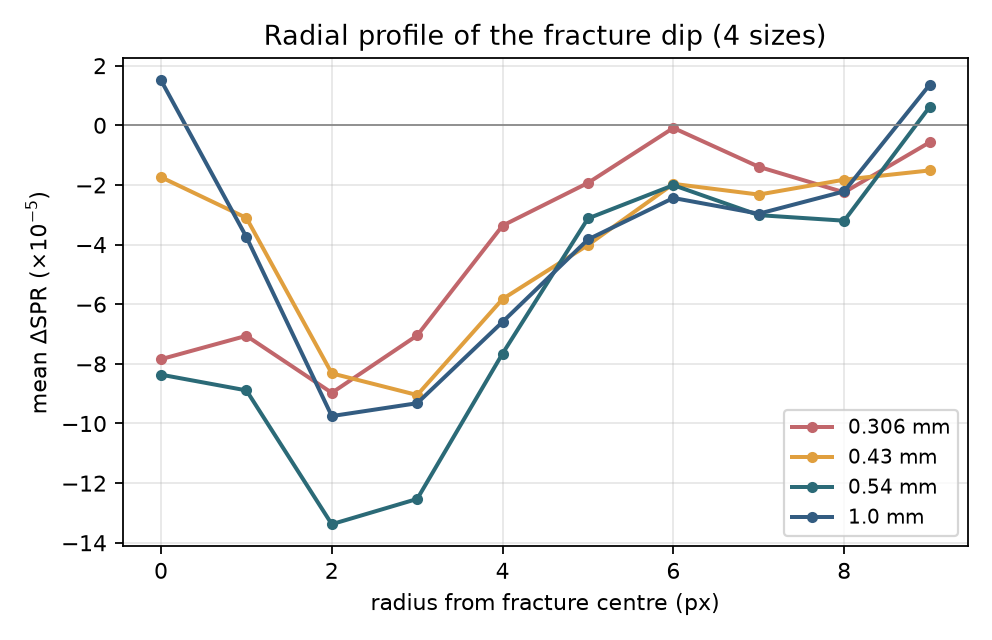
\includegraphics[width=0.66\textwidth]{fig_cl7/profiles.png}
\caption{โปรไฟล์เชิงรัศมีของ $\Delta$SPR รอบจุดร่อง; แอ่งลบที่ศูนย์กลาง (= สัญญาณรอยแตก) ปรากฏทุกขนาด
รูปทรงใกล้เคียงกัน}
\end{figure}

\subsection{สัญญาณรวมอิ่มตัว --- plateau เป็นของจริง}
\begin{keybox}
integrated $-\Delta$SPR: $5.3\to8.2\to10.4\to9.4$ ($\times10^{-3}$) --- โตจาก 0.306 ถึง 0.54~มม.\ แล้ว\textbf{คงที่}\\[2pt]
plateau test (1.0 vs 0.54, จับคู่): $\Delta=-0.99\times10^{-3}$, $t=-0.36$, $p=0.73$ $\Rightarrow$ \textbf{แยกไม่ออก}\\[2pt]
$\Rightarrow$ \textbf{สัญญาณรวมก็อิ่มตัว มิใช่แค่ค่าเฉลี่ยถูกเจือจาง} $\Rightarrow$ plateau เป็นการอิ่มตัวเชิงกายภาพจริง
\end{keybox}

\begin{figure}[h]\centering
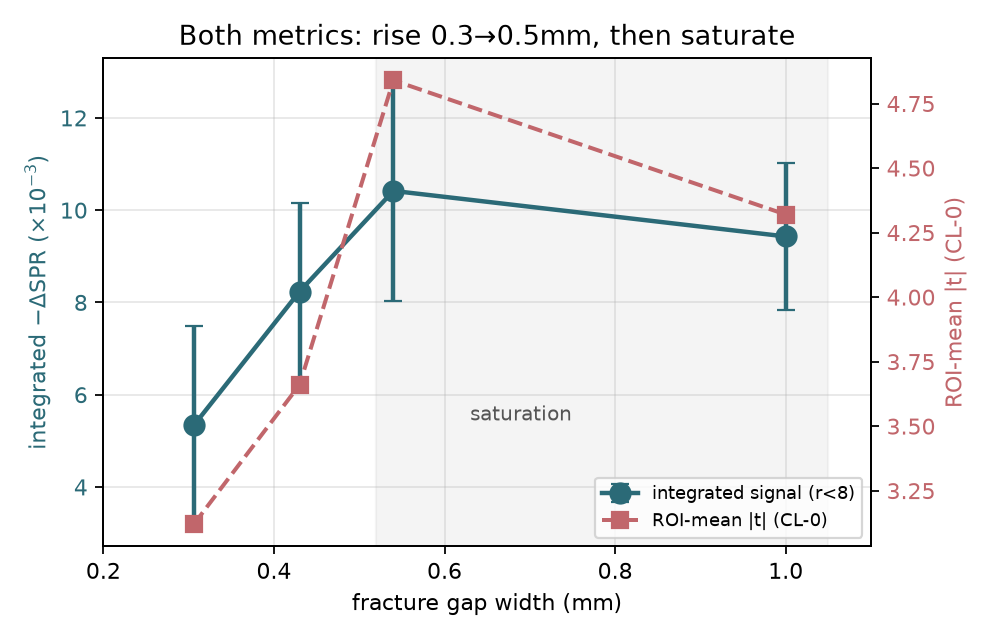
\includegraphics[width=0.66\textwidth]{fig_cl7/integrated.png}
\caption{สัญญาณรวม (แกนซ้าย, มี error bar) และ ROI-mean $|t|$ จาก CL-0 (แกนขวา) --- ทั้งคู่ขึ้นในช่วง
0.3--0.5~มม.\ แล้วเข้าสู่แถบอิ่มตัว (เทา) เหมือนกัน}
\end{figure}

\begin{figure}[h]\centering
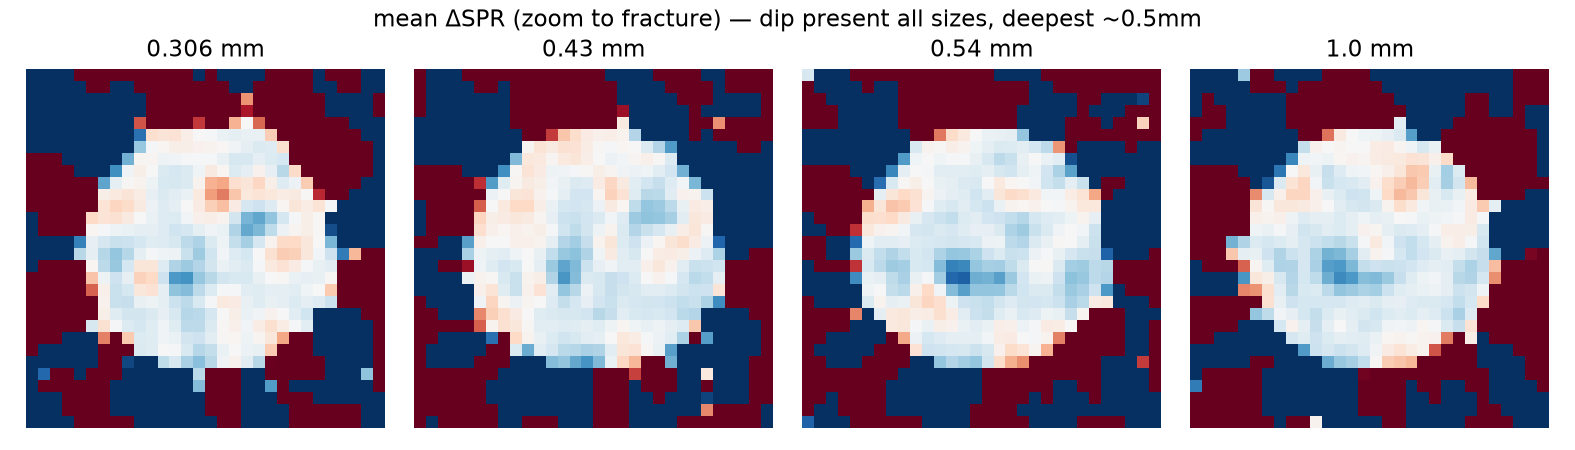
\includegraphics[width=0.95\textwidth]{fig_cl7/montage.png}
\caption{แผนที่ $\Delta$SPR เฉลี่ย (zoom ที่ร่อง) ทั้ง 4 ขนาด --- แอ่งสีน้ำเงินปรากฏทุกขนาด เข้มสุดที่ $\sim$0.5~มม.}
\end{figure}

\section{สรุปการทดสอบสมมติฐาน CL-7}
\begin{keybox}
\textbf{ปม plateau คลี่คลายแล้ว:}\ \textcolor{warn}{$\boxtimes$ \textbf{ไม่ใช่ ROI เจือจาง --- เป็นการอิ่มตัวเชิงกายภาพ}}\\[4pt]
สัญญาณรวม (integrated) ซึ่งจะโตต่อถ้าร่องกว้างขึ้นเพียงกระจายสัญญาณไปพิกเซลมากขึ้น กลับ\textbf{อิ่มตัวที่
$\sim$0.5~มม.\ เช่นเดียวกับ ROI-mean} ($p=0.73$ ที่ 0.54 vs 1.0) $\Rightarrow$ การเพิ่ม seed หรือขยาย ROI
ก็ไม่ช่วยแยก 0.54/1.0 เพราะสัญญาณกายภาพเองอิ่มตัว
\end{keybox}

\section{นัยเชิงกายภาพและต่อโครงการ}
\begin{itemize}
  \item \textbf{ขอบเขตความสามารถของ SPR:} ตรวจ\textbf{การมีอยู่}ของรอยแตกได้ไว (threshold $\sim$0.3~มม.)
        พร้อม dose--response ที่ชัดในช่วง $<0.5$~มม.\ แต่\textbf{ความไวต่อความกว้าง}อิ่มตัวเกิน $\sim$0.5~มม.
  \item \textbf{ตีความเชิงฟิสิกส์:} เมื่อช่องอากาศ ``เปิด'' พอตามแนวรังสีแล้ว การกว้างขึ้นอีกไม่เพิ่ม
        การทะลุของ primary อย่างเป็นสัดส่วน $\Rightarrow$ อัตราส่วน scatter/primary อิ่มตัว
  \item \textbf{ปิดปม CL-1 อย่างซื่อตรง:} plateau มิใช่จุดอ่อนของระเบียบวิธี แต่เป็น\textbf{คุณสมบัติจริง
        ของสัญญาณ} --- เป็นผลลัพธ์เชิงปริมาณที่มีค่าสำหรับ Phase 1 (SPR เหมาะกับการ\emph{ตรวจพบ}
        มากกว่าการ\emph{วัดความกว้าง}ของรอยแตกใหญ่)
  \item \textbf{dose--response ยังยืนยันความเป็นสัญญาณจริง} ในช่วง 0.3--0.5~มม.\ (ทั้งสองตัวชี้วัดโตตามขนาด)
\end{itemize}

\vfill
\noindent{\color{theme!45}\rule{\textwidth}{0.4pt}}\\
{\small\color{ink} รายงานเฉพาะ CL-7 ประกอบ \code{report/methodology.pdf}. วิเคราะห์บนข้อมูล CL-0 (8 seeds).
ดู CL-1 = \code{report/cl1_report.pdf}, CL-2 = \code{report/cl2_report.pdf}, ผลฐาน = \code{report/report.pdf}.}

\end{document}
